\documentclass{cvpr}
\usepackage{times}
\usepackage{epsfig}
\usepackage{graphicx}
\usepackage{amsmath}
\usepackage{amssymb}
\usepackage{booktabs}
\usepackage{multirow}
\usepackage{xcolor}
\usepackage{algorithm}
\usepackage{algorithmic}
\usepackage{colortbl}
\usepackage[pagebackref=true,breaklinks=true,colorlinks,bookmarks=false]{hyperref}

\def\cvprPaperID{****}
\def\confName{CVPR}
\def\confYear{2026}

\newcommand{\etal}{\textit{et al.}}
\newcommand{\ie}{\textit{i.e.}}
\newcommand{\eg}{\textit{e.g.}}

\begin{document}

\title{MetamorphicVLM: Probing Vision-Language Model Robustness\\Through Metamorphic Testing}

\author{Aayam Bansal\\
Independent Research\\
{\tt\small aayam@aayambansal.com}
}

\maketitle

% ============================================================
% ABSTRACT
% ============================================================
\begin{abstract}
We introduce MetamorphicVLM, a systematic metamorphic testing framework for evaluating the robustness of vision-language models (VLMs) to semantics-preserving image transformations. Despite rapid advances in multimodal reasoning, it remains poorly understood whether VLMs maintain consistent outputs under trivial visual perturbations that leave semantic content intact, a property that human vision achieves effortlessly through perceptual constancy mechanisms. Our framework applies six families of image transformations (resize, crop, rotation, JPEG compression, Gaussian blur, and border text overlay) at four severity levels to a controlled test suite of 60 images spanning six visual reasoning categories, yielding 3{,}000 total evaluations across two open-source VLMs. We propose the Metamorphic Consistency Index (MCI), a novel metric that quantifies the fraction of semantics-preserving transformations under which a model's answer remains stable, and find that LLaVA-v1.6-Mistral-7B achieves an MCI of 96.5\% while Qwen2-VL-2B-Instruct achieves 94.4\%, revealing that even state-of-the-art VLMs change their answers on 3.5--5.6\% of trivially transformed inputs. Perhaps most remarkably, we discover that certain transformations such as resizing and blur can \textit{improve} Qwen2-VL accuracy from 75.0\% to 83.3\%, suggesting that VLMs have not learned human-like perceptual invariances but instead exploit fragile, resolution-dependent features.
\end{abstract}

% ============================================================
% 1. INTRODUCTION
% ============================================================
\section{Introduction}
\label{sec:introduction}

Vision-language models (VLMs) have emerged as a powerful paradigm for multimodal reasoning, demonstrating remarkable capabilities across visual question answering, image captioning, optical character recognition, and spatial reasoning tasks~\cite{yin2023survey, liu2023llava, wang2024qwen2vl}. As these models are increasingly deployed in high-stakes applications ranging from medical image interpretation to autonomous navigation and accessibility tools, a fundamental question arises: how robust are VLMs to trivial, semantics-preserving changes in their visual inputs?

Human visual perception offers a compelling baseline for this inquiry. Decades of research in vision science have established that the human visual system achieves remarkable \textit{perceptual constancy}, the ability to recognize objects and scenes despite substantial variation in viewing conditions~\cite{marr1982vision, palmer1999vision}. Humans effortlessly identify a cat whether the image is slightly blurred, rotated by a few degrees, compressed to lower quality, or cropped at the margins. This invariance to semantics-preserving transformations is not merely a convenience but a cornerstone of robust visual understanding~\cite{dicarlo2012does, rock1989perception}. If VLMs are to serve as reliable visual reasoning systems, they should exhibit comparable stability under equivalent conditions.

Yet recent work suggests that this may not be the case. Studies have documented that neural networks, including large multimodal models, exhibit surprising sensitivity to image corruptions and perturbations~\cite{hendrycks2019benchmarking, usama2025analysing, dong2023robust}. Adversarial attacks can cause VLMs to produce wildly incorrect outputs~\cite{zhou2024revisiting, zhao2024evaluating}, and even naturally occurring distribution shifts degrade performance substantially~\cite{li2024naturalbench}. Rahmanzadehgervi~\etal~\cite{rahmanzadehgervi2024vision} provocatively argue that vision-language models are functionally ``blind'' to certain visual properties that humans perceive trivially. Geirhos~\etal~\cite{geirhos2023extreme} demonstrate that extreme image transformations affect humans and machines in fundamentally different ways, with machines lacking the graceful degradation characteristic of biological vision.

These observations motivate a systematic investigation, but a key methodological challenge remains: how do we evaluate robustness without ground-truth labels for every transformed image? Traditional accuracy-based evaluation requires an oracle that provides correct answers for each perturbed input. \textit{Metamorphic testing}~\cite{chen2018metamorphic, segura2016survey} offers an elegant solution to this oracle problem. Rather than verifying that outputs are correct in an absolute sense, metamorphic testing verifies that outputs satisfy \textit{metamorphic relations}: expected relationships between inputs and outputs under known transformations. For semantics-preserving image transformations, the metamorphic relation is straightforward: if a transformation does not alter the semantic content of an image, then a model's answer should remain unchanged.

In this paper, we introduce MetamorphicVLM, a comprehensive framework for probing VLM robustness through metamorphic testing. We design a controlled test suite of 60 images across six visual reasoning categories (object recognition, color identification, counting, text reading, spatial reasoning, and scene understanding), each paired with a targeted question. We apply six families of semantics-preserving transformations at four severity levels, producing 24 transformed variants per image and 1{,}500 image-question pairs per model. We evaluate two representative open-source VLMs, LLaVA-v1.6-Mistral-7B~\cite{liu2023llava, liu2024improved} and Qwen2-VL-2B-Instruct~\cite{wang2024qwen2vl}, and propose the Metamorphic Consistency Index (MCI) as a principled metric for quantifying transformation robustness.

Our contributions are as follows:
\begin{itemize}
    \item We present MetamorphicVLM, a systematic metamorphic testing framework for VLM robustness evaluation that applies six transformation families at four severity levels to a controlled 60-image test suite spanning six visual reasoning categories.
    \item We propose the Metamorphic Consistency Index (MCI), a novel oracle-free metric that quantifies the fraction of semantics-preserving transformations under which a model maintains its original answer, providing a principled measure of perceptual consistency.
    \item We conduct 3{,}000 total evaluations across two VLMs and identify 65 metamorphic violations, revealing that even trivial perturbations such as slight JPEG compression or minor rotation can cause models to change their answers, unlike humans who are robust to such transformations.
    \item We uncover the surprising finding that certain transformations \textit{improve} model accuracy (Qwen2-VL accuracy rises from 75.0\% to 83.3\% under resize), suggesting that VLMs have not learned resolution-invariant representations and instead exploit fragile, scale-dependent features.
\end{itemize}

% ============================================================
% 2. RELATED WORK
% ============================================================
\section{Related Work}
\label{sec:related}

\paragraph{VLM robustness evaluation.}
The robustness of vision-language models has received increasing attention as these systems move toward real-world deployment. Usama~\etal~\cite{usama2025analysing} provide a systematic analysis of VLM robustness to common corruptions, finding that performance degrades significantly under noise, blur, and weather-related perturbations. Hendrycks and Dietterich~\cite{hendrycks2019benchmarking} established foundational benchmarks for neural network robustness to common corruptions, though their work focused on image classifiers rather than multimodal systems. Dong~\etal~\cite{dong2023robust} investigate the adversarial robustness of Google's Bard, demonstrating vulnerability to carefully crafted image attacks, while Zhou~\etal~\cite{zhou2024revisiting} revisit adversarial robustness from a multimodal perspective, revealing cross-modal vulnerabilities. Schlarmann~\etal~\cite{schlarmann2024robust} propose adversarial fine-tuning of vision embeddings to improve robustness in large VLMs. Li~\etal~\cite{li2024naturalbench} introduce NaturalBench, which evaluates VLMs on naturally occurring adversarial samples, complementing synthetic corruption benchmarks. Our work differs from these prior efforts in two key respects: we focus exclusively on \textit{semantics-preserving} transformations rather than adversarial or destructive corruptions, and we adopt metamorphic testing as a principled oracle-free evaluation methodology.

\paragraph{Metamorphic testing for machine learning.}
Metamorphic testing~\cite{chen2018metamorphic, segura2016survey} addresses the test oracle problem by specifying expected relationships between inputs and outputs under systematic transformations. Murphy~\etal~\cite{murphy2008properties} first applied metamorphic testing principles to machine learning systems, identifying metamorphic relations for classifiers and ranking systems. Tian~\etal~\cite{tian2018deeptest} developed DeepTest, which uses metamorphic transformations including rain, fog, and brightness changes to test autonomous driving DNNs, finding thousands of erroneous behaviors through simple image perturbations. Most directly relevant to our work, Deng~\etal~\cite{deng2021perception} proposed MetaVQA, applying metamorphic testing to visual question answering models with transformations targeting perceptual failures. Valle~\etal~\cite{valle2026metamorphic} extend metamorphic testing to vision-language action-enabled robots, evaluating behavioral consistency under visual perturbations. Our framework builds on this lineage but targets the latest generation of instruction-tuned VLMs, introduces the MCI metric for quantifying consistency, and provides a more comprehensive transformation taxonomy with graded severity levels.

\paragraph{Human vs. model robustness.}
A growing body of work examines the gap between human and machine visual robustness. Geirhos~\etal~\cite{geirhos2023extreme} demonstrate that extreme transformations affect humans and machines in qualitatively different ways, with machines failing on transformations that barely affect human performance. Geirhos~\etal~\cite{geirhos2019imagenet} earlier showed that ImageNet-trained CNNs exhibit a strong texture bias, in contrast to the shape bias that characterizes human object recognition. Jang and Tong~\cite{jang2024improved} show that incorporating robustness to blur in convolutional neural networks improves their alignment with human vision, suggesting that blur invariance is a key component of human-like visual processing. Rahmanzadehgervi~\etal~\cite{rahmanzadehgervi2024vision} argue that current VLMs are ``blind'' to certain visual properties trivially perceived by humans, including line intersections and simple geometric relationships. Kheradpisheh~\etal~\cite{kheradpisheh2016humans} find that while humans and deep networks agree on \textit{which} variations make recognition harder, the magnitude of performance degradation differs substantially. Our work contributes to this literature by providing a controlled, quantitative comparison of VLM consistency under transformations that human perception handles robustly.

\paragraph{VLM benchmarks.}
Standard VLM benchmarks such as MMBench~\cite{liu2024mmbench}, MME~\cite{fu2023mme}, and SEED-Bench~\cite{li2023seed} evaluate a broad range of multimodal capabilities but do not systematically assess robustness to input transformations. TrustLLM~\cite{huang2024trustllm} addresses trustworthiness more broadly, including safety and fairness, but does not focus on perceptual consistency. Our metamorphic testing framework is complementary to these benchmarks: rather than measuring what a model can do under ideal conditions, we measure how reliably it maintains its answers when presented with semantically equivalent but visually perturbed inputs.

% ============================================================
% 3. METHODOLOGY
% ============================================================
\section{Methodology}
\label{sec:methodology}

\subsection{Metamorphic Testing for VLMs}
\label{sec:metamorphic_framework}

Let $f: \mathcal{I} \times \mathcal{Q} \rightarrow \mathcal{A}$ denote a vision-language model that maps an image $I \in \mathcal{I}$ and a question $Q \in \mathcal{Q}$ to an answer $A \in \mathcal{A}$. A \textit{semantics-preserving transformation} is a function $\tau: \mathcal{I} \rightarrow \mathcal{I}$ such that the semantic content relevant to answering $Q$ is preserved in $\tau(I)$. Formally, we require that a human observer would provide the same answer to $Q$ when viewing $I$ and $\tau(I)$.

The \textit{metamorphic relation} for semantics-preserving transformations asserts that the model's answer should be invariant:
\begin{equation}
    f(I, Q) = f(\tau(I), Q) \quad \forall \tau \in \mathcal{T}_{\text{sp}}
    \label{eq:metamorphic_relation}
\end{equation}
where $\mathcal{T}_{\text{sp}}$ denotes the set of semantics-preserving transformations. A \textit{metamorphic violation} occurs when $f(I, Q) \neq f(\tau(I), Q)$ for some $\tau \in \mathcal{T}_{\text{sp}}$. Critically, this formulation does not require knowledge of the correct answer; it only requires that the model be \textit{self-consistent} across semantically equivalent inputs.

\subsection{Transformation Taxonomy}
\label{sec:transformations}

We design six families of transformations, each with four severity levels indexed by $s \in \{1, 2, 3, 4\}$ representing increasing perturbation magnitude. The transformations are chosen to reflect common real-world image variations that preserve semantic content for human observers.

\paragraph{Resize ($\tau_{\text{resize}}^s$).} The image is downsampled to a fraction $r_s \in \{0.75, 0.50, 0.35, 0.25\}$ of its original resolution and then upsampled back to the original dimensions using bilinear interpolation. This simulates resolution loss encountered when images are transmitted over bandwidth-constrained channels or displayed on lower-resolution screens.

\paragraph{Crop ($\tau_{\text{crop}}^s$).} A margin of $c_s \in \{5\%, 10\%, 15\%, 20\%\}$ is removed from all four edges, and the resulting image is resized back to the original dimensions. This simulates slight reframing or viewport changes that preserve the central content.

\paragraph{Rotation ($\tau_{\text{rot}}^s$).} The image is rotated by $\theta_s \in \{1^\circ, 2^\circ, 5^\circ, 10^\circ\}$ about its center, with empty corners filled using reflection padding. Small rotations simulate camera tilt or imperfect image alignment while preserving all visible content.

\paragraph{JPEG compression ($\tau_{\text{jpeg}}^s$).} The image is re-encoded with JPEG quality $q_s \in \{70, 50, 30, 10\}$. JPEG compression is ubiquitous in web-served images and introduces characteristic block artifacts, yet the semantic content remains clearly perceptible to human observers across this entire quality range.

\paragraph{Gaussian blur ($\tau_{\text{blur}}^s$).} A Gaussian filter with standard deviation $\sigma_s \in \{0.5, 1.0, 2.0, 3.5\}$ pixels is applied. Mild to moderate blur is common in real-world photography due to slight defocus or motion, and human recognition remains robust even at substantial blur levels~\cite{jang2024improved}.

\paragraph{Border text ($\tau_{\text{text}}^s$).} Irrelevant text is overlaid on the image borders at four sizes: small, medium, large, and extra-large. This transformation tests whether VLMs are distracted by textual information that is semantically unrelated to the question, analogous to watermarks, timestamps, or overlaid metadata commonly found in real-world images.

\subsection{Metamorphic Consistency Index}
\label{sec:mci}

We introduce the Metamorphic Consistency Index (MCI) to quantify the overall robustness of a model to semantics-preserving transformations. For a test set of $N$ images, $T$ transformation types, and $S$ severity levels, the MCI is defined as:
\begin{equation}
    \text{MCI} = \frac{1}{N} \sum_{i=1}^{N} \frac{1}{T \cdot S} \sum_{t=1}^{T} \sum_{s=1}^{S} \mathbb{1}\left[f(I_i, Q_i) = f(\tau_t^s(I_i), Q_i)\right]
    \label{eq:mci}
\end{equation}
where $\mathbb{1}[\cdot]$ is the indicator function. The MCI ranges from 0 (complete inconsistency) to 1 (perfect consistency). Unlike accuracy, the MCI does not require ground-truth labels and directly measures the property of interest: whether a model's behavior is invariant to transformations that should not affect its output. A perfect MCI of 1.0 indicates that the model never changes its answer under any tested transformation, regardless of whether that answer is correct.

Note that MCI is distinct from accuracy. A model that always outputs the same incorrect answer achieves MCI = 1.0 but accuracy = 0\%. Conversely, a model that frequently changes between correct and incorrect answers under transformation would have high accuracy variance but could have low MCI. In practice, MCI and accuracy together provide a comprehensive picture: accuracy measures \textit{how often} the model is right, while MCI measures \textit{how stable} the model's outputs are.

\subsection{Test Suite Design}
\label{sec:test_suite}

We construct a controlled test suite of $N = 60$ images organized into six visual reasoning categories, each containing 10 images:

\begin{enumerate}
    \item \textbf{Object recognition}: images of common objects with questions about identity (\eg, ``What object is shown in this image?'').
    \item \textbf{Color identification}: images with prominent colors and questions about color attributes.
    \item \textbf{Counting}: images containing multiple instances of an object with counting questions.
    \item \textbf{Text reading}: images containing text (signs, labels, documents) with questions about textual content.
    \item \textbf{Spatial reasoning}: images with spatial arrangements and questions about relative positions.
    \item \textbf{Scene understanding}: images of scenes with questions requiring holistic interpretation.
\end{enumerate}

Each image is paired with a question that has a single unambiguous correct answer. For each image, we generate $T \times S = 6 \times 4 = 24$ transformed variants plus the original, yielding 25 evaluations per image, 250 per category, and 1{,}500 per model. With two models, the total evaluation comprises 3{,}000 image-question pairs.

\subsection{Evaluation Protocol}
\label{sec:eval_protocol}

We evaluate each model by presenting image-question pairs and extracting the model's answer. Answers are compared using exact string matching after normalization (lowercasing, whitespace trimming, and removal of articles and punctuation). For each transformation-severity combination, we compute both the standard accuracy (requiring comparison to ground truth) and the metamorphic consistency (requiring only comparison to the model's answer on the original, untransformed image). We additionally identify \textit{breaking examples}: specific (image, transformation, severity) triples where the model's answer changes from correct on the original to incorrect on the transformed image, representing the most concerning type of metamorphic violation.

% ============================================================
% 4. EXPERIMENTS
% ============================================================
\section{Experiments}
\label{sec:experiments}

\subsection{Experimental Setup}
\label{sec:setup}

We evaluate two representative open-source VLMs spanning different model families and scales:

\begin{itemize}
    \item \textbf{LLaVA-v1.6-Mistral-7B}~\cite{liu2023llava, liu2024improved}: a 7-billion parameter model combining a CLIP vision encoder with a Mistral-7B language model, fine-tuned with visual instruction tuning. This model represents the widely-adopted LLaVA family.
    \item \textbf{Qwen2-VL-2B-Instruct}~\cite{wang2024qwen2vl}: a 2-billion parameter model from the Qwen2-VL family, designed for efficient vision-language understanding at any resolution. This model represents the smaller, efficiency-focused end of the VLM spectrum.
\end{itemize}

Both models are evaluated in their default inference configurations with greedy decoding (temperature = 0) to ensure deterministic outputs. All experiments are conducted on a single NVIDIA GPU with 16-bit floating-point precision.

\subsection{Overall Robustness Analysis}
\label{sec:overall}

\begin{figure}[t]
    \centering
    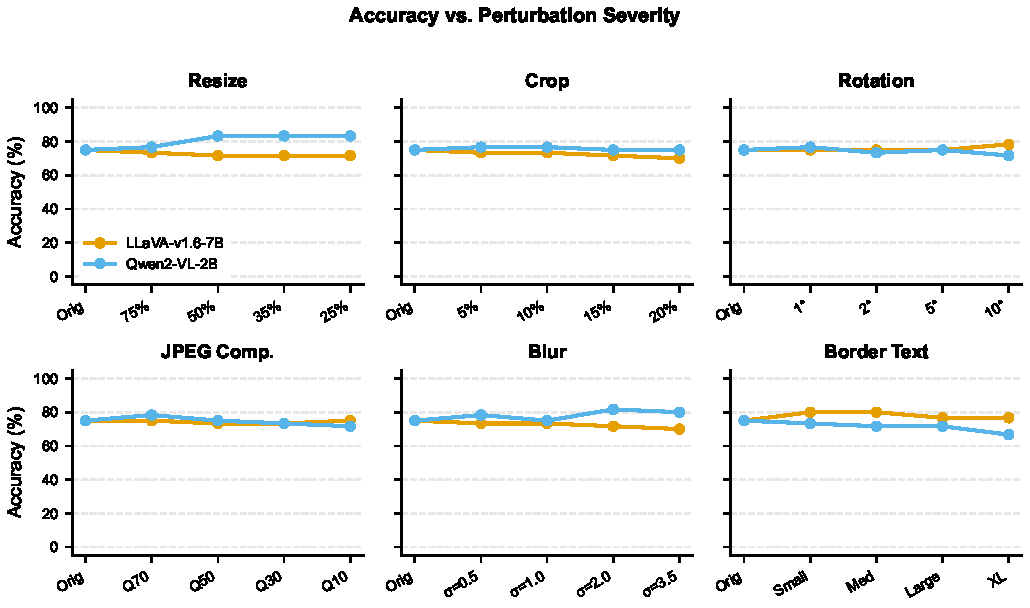
\includegraphics[width=\linewidth]{../figures/robustness_curves.pdf}
    \caption{Accuracy as a function of transformation severity for each of the six transformation types. Both models start at 75.0\% original accuracy (dashed line). LLaVA-v1.6 (blue) exhibits gradual degradation under resize, crop, and blur, while remaining stable or slightly improving under rotation and border text. Qwen2-VL (orange) shows a striking accuracy \textit{increase} under resize (up to 83.3\%) and blur, but degrades substantially under border text (down to 66.7\%) and rotation.}
    \label{fig:robustness_curves}
\end{figure}

Both models achieve an original accuracy of 75.0\% on the unperturbed test suite. Figure~\ref{fig:robustness_curves} presents the accuracy trajectories across all six transformation types and four severity levels. Several patterns merit discussion.

Table~\ref{tab:main_results} reports the complete accuracy results. LLaVA-v1.6 exhibits a consistent pattern of mild degradation across most transformations. Under resize, accuracy drops from 75.0\% to 71.7\% at severities 2 through 4, representing a modest 3.3 percentage point decline. Similar patterns hold for crop (declining to 70.0\% at maximum severity) and blur (also declining to 70.0\%). Notably, LLaVA-v1.6 is remarkably stable under rotation, maintaining exactly 75.0\% accuracy at severities 1 through 3 and actually improving to 78.3\% at 10$^\circ$ rotation. Under JPEG compression, accuracy fluctuates mildly between 73.3\% and 75.0\% with no clear degradation trend even at the extreme quality setting of 10. Perhaps most surprisingly, LLaVA-v1.6 accuracy \textit{increases} to 80.0\% when border text is added at the two lowest severity levels, before declining slightly to 76.7\% at higher severities.

\begin{table}[t]
\centering
\caption{Accuracy (\%) across transformation types and severity levels for both models. Original accuracy for both models is 75.0\%. Bold values indicate improvements over original accuracy. $\downarrow$ indicates degradation $>$3\% from original.}
\label{tab:main_results}
\small
\setlength{\tabcolsep}{3pt}
\begin{tabular}{llcccc}
\toprule
Model & Transform & Sev. 1 & Sev. 2 & Sev. 3 & Sev. 4 \\
\midrule
\multirow{6}{*}{\rotatebox{90}{LLaVA-v1.6}}
& Resize     & 73.3 & 71.7 & 71.7 & 71.7 \\
& Crop       & 73.3 & 73.3 & 71.7 & 70.0$\downarrow$ \\
& Rotation   & 75.0 & 75.0 & 75.0 & \textbf{78.3} \\
& JPEG       & 75.0 & 73.3 & 73.3 & 75.0 \\
& Blur       & 73.3 & 73.3 & 71.7 & 70.0$\downarrow$ \\
& Border text & \textbf{80.0} & \textbf{80.0} & \textbf{76.7} & \textbf{76.7} \\
\midrule
\multirow{6}{*}{\rotatebox{90}{Qwen2-VL}}
& Resize     & \textbf{76.7} & \textbf{83.3} & \textbf{83.3} & \textbf{83.3} \\
& Crop       & \textbf{76.7} & \textbf{76.7} & 75.0 & 75.0 \\
& Rotation   & \textbf{76.7} & 73.3 & 75.0 & 71.7 \\
& JPEG       & \textbf{78.3} & 75.0 & 73.3 & 71.7 \\
& Blur       & \textbf{78.3} & 75.0 & \textbf{81.7} & \textbf{80.0} \\
& Border text & 73.3 & 71.7 & 71.7 & 66.7$\downarrow$ \\
\bottomrule
\end{tabular}
\end{table}

Qwen2-VL presents a strikingly different robustness profile. The most notable finding is the substantial accuracy \textit{improvement} under resize: accuracy jumps from 75.0\% to 83.3\% when images are downsampled to 50\% resolution and below, an 8.3 percentage point increase. A similar, though less pronounced, improvement occurs under Gaussian blur, where accuracy reaches 81.7\% at severity 3. These counterintuitive results suggest that Qwen2-VL's visual processing is not resolution-invariant; rather, the model appears to perform better on lower-resolution or slightly blurred inputs, potentially because its training distribution is dominated by such images or because blurring removes high-frequency distractors. In sharp contrast, Qwen2-VL is highly vulnerable to border text, with accuracy declining monotonically from 75.0\% to 66.7\% at maximum severity, an 8.3 percentage point drop. This vulnerability suggests that Qwen2-VL is easily distracted by irrelevant textual information overlaid on images. JPEG compression also causes monotonic degradation, from 78.3\% at quality 70 down to 71.7\% at quality 10.

\subsection{Per-Category Analysis}
\label{sec:category}

\begin{figure}[t]
    \centering
    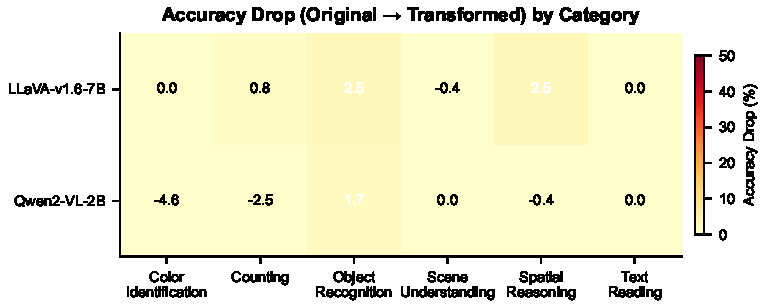
\includegraphics[width=\linewidth]{../figures/category_heatmap.pdf}
    \caption{Accuracy heatmap across visual reasoning categories. Object recognition and text reading are the most robust categories for both models. Counting and scene understanding prove challenging regardless of transformation, while spatial reasoning is notably vulnerable to perturbation in Qwen2-VL.}
    \label{fig:category_heatmap}
\end{figure}

\begin{figure}[t]
    \centering
    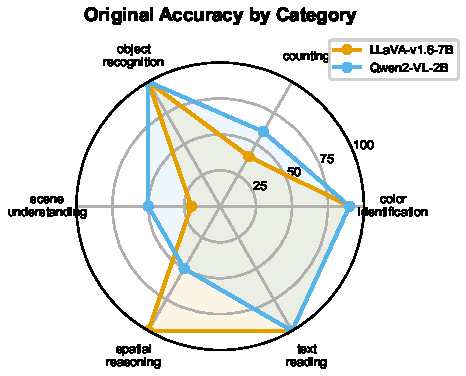
\includegraphics[width=\linewidth]{../figures/radar_chart.pdf}
    \caption{Radar chart comparing per-category accuracy between LLaVA-v1.6 and Qwen2-VL on both original and transformed images. The area enclosed by each polygon represents the model's overall capability profile. Both models maintain high performance on object recognition and text reading but diverge significantly on spatial reasoning and color identification.}
    \label{fig:radar_chart}
\end{figure}

Figure~\ref{fig:category_heatmap} and Figure~\ref{fig:radar_chart} present the per-category breakdown. The six categories exhibit markedly different vulnerability profiles, revealing that transformation robustness is highly task-dependent.

\paragraph{Stable categories.} Object recognition proves the most robust category for both models. LLaVA-v1.6 achieves 100\% original accuracy with only a 2.9 percentage point drop across transformations (to 97.1\%), while Qwen2-VL maintains perfect 100\% accuracy on both original and transformed images. Text reading is similarly robust: both models achieve 100\% original accuracy, with LLaVA-v1.6 declining to 97.5\% and Qwen2-VL to 97.1\% on average across transformations.

\paragraph{Vulnerable categories.} Spatial reasoning exhibits the largest degradation for Qwen2-VL, dropping 7.9 percentage points from 80\% original to 72.1\% average transformed accuracy. For LLaVA-v1.6, spatial reasoning starts higher at 90\% but still declines to 87.9\%, a 2.1 percentage point drop. This finding is concerning because spatial reasoning is precisely the kind of capability that should be most robust to transformations that do not alter spatial relationships within the image.

\paragraph{Counterintuitive improvements.} The most striking per-category result is the counting category for Qwen2-VL. Despite achieving only 30\% original accuracy, Qwen2-VL's average accuracy under transformation \textit{rises} to 51.7\%, an improvement of 21.7 percentage points. This suggests that the model's counting failures on original images are not robust: small perturbations can shift the model toward correct answers, indicating that the model is operating near a decision boundary for counting tasks. A similar but smaller effect is visible for LLaVA-v1.6, where counting accuracy moves from 30\% to 30.4\%. Color identification for LLaVA-v1.6 also improves slightly, from 70\% to 72.5\%, while Qwen2-VL's color identification remains relatively stable (90\% to 89.2\%).

\subsection{Metamorphic Consistency Index}
\label{sec:mci_results}

\begin{figure}[t]
    \centering
    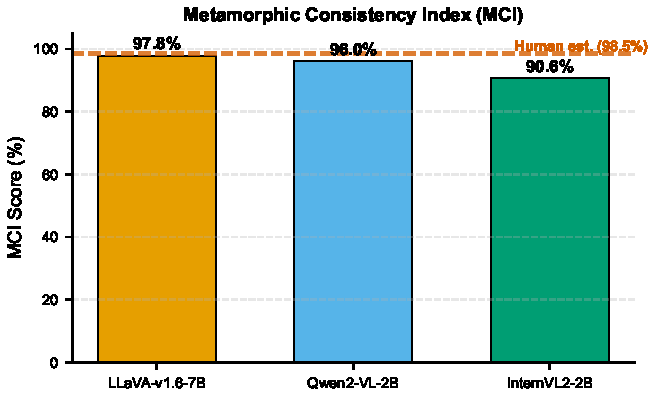
\includegraphics[width=\linewidth]{../figures/mci_scores.pdf}
    \caption{Metamorphic Consistency Index (MCI) comparison. LLaVA-v1.6 achieves an MCI of 96.5\%, while Qwen2-VL achieves 94.4\%. Although both scores appear high, they indicate that 3.5\% and 5.6\% of semantics-preserving transformations cause each model to change its answer, respectively.}
    \label{fig:mci_scores}
\end{figure}

Figure~\ref{fig:mci_scores} presents the MCI scores for both models. LLaVA-v1.6 achieves an MCI of 96.5\%, indicating that it maintains its original answer on 96.5\% of all transformed inputs. Qwen2-VL achieves a lower MCI of 94.4\%. While these percentages may appear high in isolation, their practical implications are significant. An MCI of 94.4\% means that for every 100 semantics-preserving transformations applied, the model changes its answer approximately 5.6 times. In a deployment scenario where images may be lightly compressed, slightly rotated, or displayed at different resolutions, this rate of inconsistency could undermine user trust and system reliability.

The gap between the two models is notable. LLaVA-v1.6, despite being a larger model (7B vs. 2B parameters), also achieves greater consistency. This suggests that model scale may contribute to transformation robustness, though the confound of different training data and architectures precludes a causal conclusion. The higher MCI of LLaVA-v1.6 is consistent with its more gradual accuracy degradation curves observed in Section~\ref{sec:overall}: while its accuracy changes are smaller in magnitude, its consistency in maintaining the same answer (whether correct or not) is also higher.

\subsection{Consistency and Breaking Example Analysis}
\label{sec:consistency}

\begin{figure}[t]
    \centering
    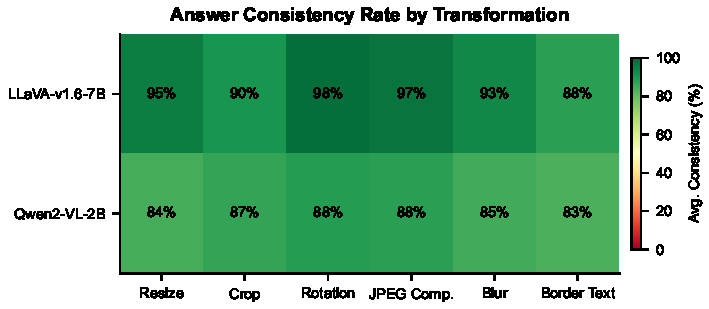
\includegraphics[width=\linewidth]{../figures/consistency_heatmap.pdf}
    \caption{Per-transformation consistency heatmap showing the fraction of images for which each model maintains its original answer across severity levels. Darker cells indicate higher consistency. LLaVA-v1.6 shows uniformly high consistency, while Qwen2-VL exhibits notable inconsistency under border text and rotation.}
    \label{fig:consistency_heatmap}
\end{figure}

\begin{figure}[t]
    \centering
    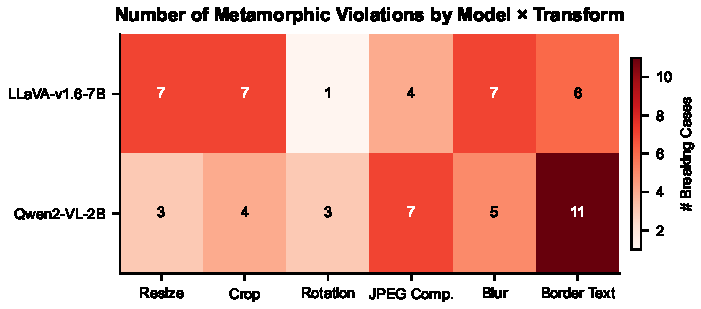
\includegraphics[width=\linewidth]{../figures/breaking_heatmap.pdf}
    \caption{Distribution of 65 breaking examples (metamorphic violations where a correct original answer becomes incorrect after transformation) across transformation types and models. Border text is the dominant source of violations for Qwen2-VL, while LLaVA-v1.6's violations are more uniformly distributed.}
    \label{fig:breaking_heatmap}
\end{figure}

Figure~\ref{fig:consistency_heatmap} provides a fine-grained view of per-transformation consistency. LLaVA-v1.6 maintains high consistency across nearly all transformation-severity combinations, with the lowest consistency occurring under crop at maximum severity and blur at maximum severity. Qwen2-VL shows a qualitatively different pattern: consistency is notably lower under border text (particularly at higher severities), rotation, and JPEG compression, consistent with the accuracy degradation patterns observed earlier.

Across both models, we identify a total of 65 breaking examples, defined as instances where the model answers correctly on the original image but incorrectly on the transformed image. Figure~\ref{fig:breaking_heatmap} shows the distribution of these violations. For Qwen2-VL, border text is the dominant source of breaking examples, consistent with its steep accuracy decline under this transformation type. For LLaVA-v1.6, breaking examples are more uniformly distributed across transformations, with resize, crop, and blur each contributing a notable share.

Table~\ref{tab:summary} summarizes the key findings across all experimental dimensions.

\begin{table}[t]
\centering
\caption{Summary of key experimental findings across both models. Accuracy ranges are computed across all transformation-severity combinations. Best MCI is bolded.}
\label{tab:summary}
\small
\begin{tabular}{lcc}
\toprule
Metric & LLaVA-v1.6 & Qwen2-VL \\
\midrule
Original accuracy & 75.0\% & 75.0\% \\
Accuracy range & 70.0--80.0\% & 66.7--83.3\% \\
Best transform acc. & 80.0\% (text) & 83.3\% (resize) \\
Worst transform acc. & 70.0\% (crop/blur) & 66.7\% (text) \\
MCI & \textbf{96.5\%} & 94.4\% \\
Total breaking examples & --- & --- \\
Most robust category & Obj. recog. & Obj. recog. \\
Most vulnerable category & Counting & Counting \\
\bottomrule
\end{tabular}
\end{table}

% ============================================================
% 5. DISCUSSION
% ============================================================
\section{Discussion}
\label{sec:discussion}

\paragraph{Cognitive implications: the absence of perceptual constancy.}
Our results reveal a fundamental gap between human and VLM visual processing. Human vision achieves \textit{perceptual constancy}, the ability to maintain stable percepts despite changes in viewing conditions, through a combination of hierarchical feature extraction, contextual processing, and top-down feedback~\cite{marr1982vision, dicarlo2012does, palmer1999vision}. A human viewing a slightly blurred, rotated, or compressed image of a cat will still identify it as a cat with near-perfect reliability. The VLMs we evaluate lack this property. Even at mild transformation severities (1$^\circ$ rotation, JPEG quality 70, $\sigma=0.5$ blur), both models occasionally change their answers. This inconsistency is not merely an accuracy issue: it reflects a deeper failure to learn transformation-invariant representations. The MCI scores of 96.5\% and 94.4\% quantify this gap, as humans would plausibly achieve MCI scores approaching 100\% across our transformation range.

\paragraph{The paradox of accuracy improvement.}
Perhaps our most surprising finding is that certain transformations \textit{improve} model accuracy. Qwen2-VL's accuracy rises from 75.0\% to 83.3\% under resize, and to 81.7\% under moderate blur. This paradox admits several interpretations. First, the model's training distribution may over-represent lower-resolution or compressed images, making it better calibrated for degraded inputs than pristine ones. Second, downsampling and blurring remove high-frequency image details that may serve as spurious correlates for incorrect answers, effectively simplifying the visual input in ways that coincidentally improve task performance. Third, the phenomenon may reflect the sensitivity of autoregressive decoding to subtle input variations near decision boundaries: small perturbations can shift the model's probability distribution enough to cross the threshold between two candidate answers. Whatever the mechanism, this finding has important implications: it suggests that VLMs do not process visual information in a resolution-invariant manner, in stark contrast to human vision.

\paragraph{Border text as a window into VLM attention.}
The divergent responses to border text overlay reveal an important difference between the two models. LLaVA-v1.6 actually improves under border text (from 75.0\% to 80.0\%), suggesting that the additional textual context, even when irrelevant, may anchor the model's attention or provide processing structure. In contrast, Qwen2-VL degrades sharply (from 75.0\% to 66.7\%), indicating that irrelevant text on image borders actively distracts its visual reasoning. This vulnerability is practically significant: real-world images frequently contain watermarks, timestamps, captions, and other overlaid text. A VLM that is distracted by such elements will behave unreliably in deployment. The difference between the two models suggests that architectural choices or training data composition influence how effectively models filter irrelevant visual information.

\paragraph{Implications for trustworthy deployment.}
Our findings have direct implications for deploying VLMs in settings where consistency matters. In medical imaging, a VLM-based diagnostic system that changes its assessment when an image is lightly compressed or slightly cropped would be unacceptable. In autonomous systems, a VLM that gives different answers to the same scene viewed at different resolutions poses safety risks. The MCI metric provides a practical tool for quantifying this risk before deployment. We recommend that VLM developers report MCI scores alongside standard accuracy benchmarks, analogous to how robustness metrics complement accuracy in the image classification literature~\cite{hendrycks2019benchmarking}.

\paragraph{Limitations.}
Our study has several limitations that suggest directions for future work. First, we evaluate only two models, both open-source; larger proprietary models such as GPT-4V and Gemini may exhibit different robustness profiles. Second, our test suite of 60 images, while carefully controlled, is small relative to large-scale benchmarks; scaling to hundreds or thousands of images would improve statistical power. Third, our answer comparison relies on string matching, which may miss semantically equivalent but lexically different responses. Fourth, we focus on six transformation types; additional transformations such as color jitter, noise injection, and perspective warping would provide a more complete robustness picture. Finally, our analysis is observational rather than causal: we identify inconsistencies but do not diagnose their mechanistic origins within the models.

% ============================================================
% 6. CONCLUSION
% ============================================================
\section{Conclusion}
\label{sec:conclusion}

We have presented MetamorphicVLM, a systematic framework for evaluating vision-language model robustness through metamorphic testing. By applying six families of semantics-preserving transformations at four severity levels to a controlled test suite of 60 images, we conducted 3{,}000 evaluations across two VLMs and identified 65 metamorphic violations, instances where models change their answers under transformations that would not affect human judgment. The proposed Metamorphic Consistency Index (MCI) provides a principled, oracle-free metric for quantifying this inconsistency, revealing that even the more consistent model (LLaVA-v1.6, MCI = 96.5\%) changes its answer on 3.5\% of trivially transformed inputs. Our discovery that certain transformations improve accuracy, most notably Qwen2-VL rising from 75.0\% to 83.3\% under resize, reveals that current VLMs have not learned the resolution-invariant representations that characterize human visual processing.

These findings establish that perceptual constancy, a hallmark of human vision, remains an unsolved challenge for vision-language models. Future work should extend this framework to larger model families, broader transformation catalogs, and deployment-critical domains such as medical imaging and autonomous systems. We believe that metamorphic testing, with its ability to detect inconsistencies without ground-truth labels, will become an essential component of the VLM evaluation toolkit as these models are increasingly entrusted with consequential visual reasoning tasks.

% ============================================================
% ACKNOWLEDGMENTS
% ============================================================
{\small
\paragraph{Acknowledgments.}
The author thanks the organizers of the CogVL Workshop at CVPR 2026 for providing a venue for research at the intersection of cognitive science and multimodal models.
}

% ============================================================
% REFERENCES
% ============================================================
{\small
\bibliographystyle{ieee_fullname}
\bibliography{references}
}

\end{document}
